\subsection{Evaluation Strategies}
Programming language behaviour is heavily dependent on the evaluation strategy employed. Conventionally two such strategies are prominent in the literature\cite{DBLP:journals/cl/Tremblay-lenient}; \textit{strict} (also called eager) and \textit{non-strict} (commonly known as lazy, though this is not entirely accurate). \cite{DBLP:journals/cl/Tremblay-lenient} suggests a \textit{lenient} evaluated language. This strategy is non-strict, but not lazy, which places it in-between eager and lazy\cite{DBLP:journals/cl/Tremblay-lenient}. This intermediary position means that the lenient strategy benefits from both eager and lazy advantages. According to literature lenient evaluation lends itself to implicit parallelism\cite{DBLP:journals/cl/Tremblay-parallel}. This section will explore the three strategies and clarify the distinctions between them.

In Sweeney's discussion of the game-programming language of tomorrow, he underlines that it should make use of the lenient evaluation strategy\cite{theNextMainstreanProgrammingLanguage}. The reason for this is that eager evaluation strategy is too limiting and lazy evaluation is too costly. Sweeney also underlines that the compiler of this new language should be capable of optimising pieces of code to use eager evaluation, whenever it is more optimal.

\subsubsection{Strict Evaluation}
Strict evaluation, often called eager evaluation, is a prominent evaluation strategy in traditional programming languages. The defining feature of the strategy lies in the handling of function parameters. Eager evaluation requires fully evaluated parameters before a function may be evaluated\cite[p.~103]{huttel2010transitions}, however this is not the only requirement. Depending on the choice of parameter passing approach, the evaluation strategy may also be affected. Chief among eager parameter passing approaches are call-by-value and call-by-reference. In the case of call-by-value a parameter must be evaluated and its result passed to the function. On the other hand call-by-reference has the same requirement, but instead the memory address of the result is passed to the function.

\subsubsection{Non-strict Evaluation}
Contrary to strict evaluation, non-strict evaluation does not require parameter evaluation until they are needed\cite{hudak1989conception}. This strategy is often implemented using call-by-name or call-by-need parameter-passing approaches. This strategy affords the programmers more expressive power\cite{bird1997more} and allows for infinite data structures and non-terminating functions\cite[p.~103]{huttel2010transitions}. The parameter passing approaches state that parameter evaluation is delayed until they are called, therefore unused parameters need not be calculated at all.

\subsubsection{Lenient Evaluation}
The lenient evaluation strategy does not restrict the order of parameter evaluation. The only requirement is that the variables are available when they are needed, or in other words that the data dependencies are satisfied. Parameter passing approaches in this strategy often make extensive use of parallelism and concurrency techniques, due to the inherent parallelisability of lenient evaluation\cite{DBLP:journals/cl/Tremblay-parallel}.

The most notable instantiation of this evaluation strategy is call-by-future\cite{baker1977incremental}. In this implementation the main thread of the program executes the program and every time it encounters a function invocation, it spawns a future for each argument to the function. The main thread then continues to execute the function-body, synchronising with the futures as arguments are needed in the function-body. This has the result that functions and arguments are computed concurrently. The parallelisability of programs may vary greatly, depending on how the program is written and what it is intended to do. Therefore, we examine static analysis methods to determine when to parallelise.

A visualisation of parallelism in the different evaluation strategies can be seen in \figref{eval-para}. Here two cases are compared: a summation of a binary tree (\figref{eval-para-1}) and sorting and summation of a list (\figref{eval-para-2}). The X axis represents time and the Y axis represents the number items that can be computed in parallel at that given point in time.

\begin{figure}[H]%
\alignCenter{\begin{minipage}[c]{1.2\textwidth}%
\begin{subfigure}{.45\textwidth}%
  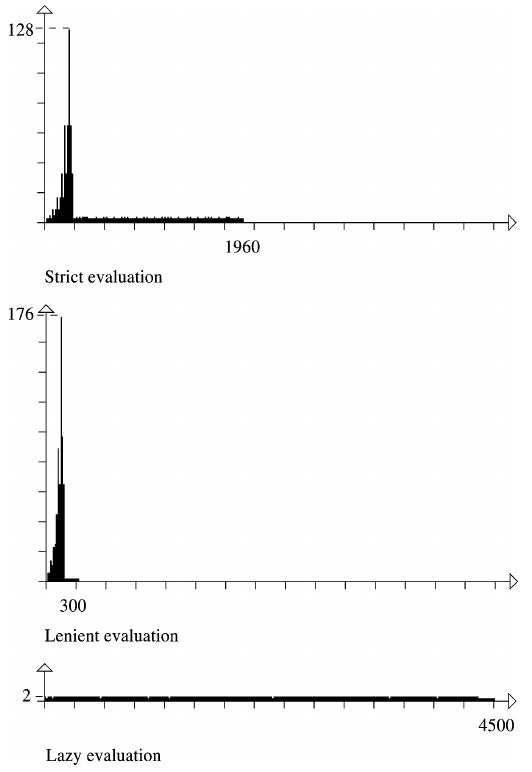
\includegraphics[width=1.1\textwidth]{00-images/eval-para-1.png}%
  \caption{Parallelism profiles for computing the sum of the leaves of a binary tree}%
  \label{fig:eval-para-1}%
\end{subfigure}%
\hfill
\begin{subfigure}{.45\textwidth}%
  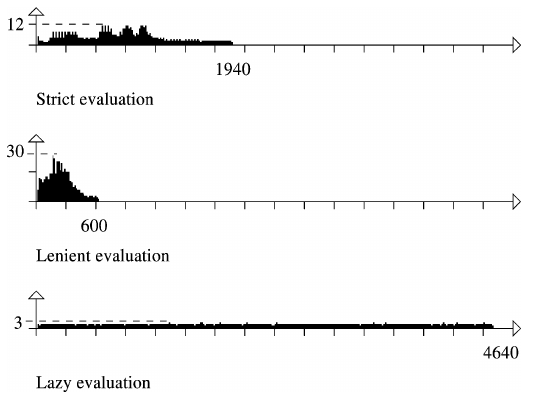
\includegraphics[width=1.1\textwidth]{00-images/eval-para-2.png}%
  \caption{Parallelism profiles for sorting a list and computing its sum}
  \label{fig:eval-para-2}%
\end{subfigure}%
\end{minipage}}
\caption{Parallelism profiles for evaluation strategies\cite{DBLP:journals/cl/Tremblay-parallel}}%
\label{fig:eval-para}%
\end{figure}%
